%--------------------------------------------------------
\begin{frame}
\frametitle{Baryon Enhancement}

\begin{columns}[T,onlytextwidth]

%--------------------------------------------------------
\column{0.38\textwidth}

\small

\textbf{Observable}

\[
\frac{p}{\pi}(p_T)
=
\frac{dN_p/dp_T}{dN_\pi/dp_T}
\]

\vspace{0.25cm}

\textbf{Enhancement region}

\[
2 \lesssim p_T \lesssim 5~{\rm GeV}/c
\]

\vspace{0.4cm}

\begin{itemize}
    \item Larger in central Pb--Pb.
    \item Driven by collective radial flow.
    \item Sensitive to QGP hadronization.
\end{itemize}

{\tiny
Data source: HEPData\\
10.17182/HEPData-ins1759506-v1.
}
%--------------------------------------------------------
\column{0.60\textwidth}

\centering

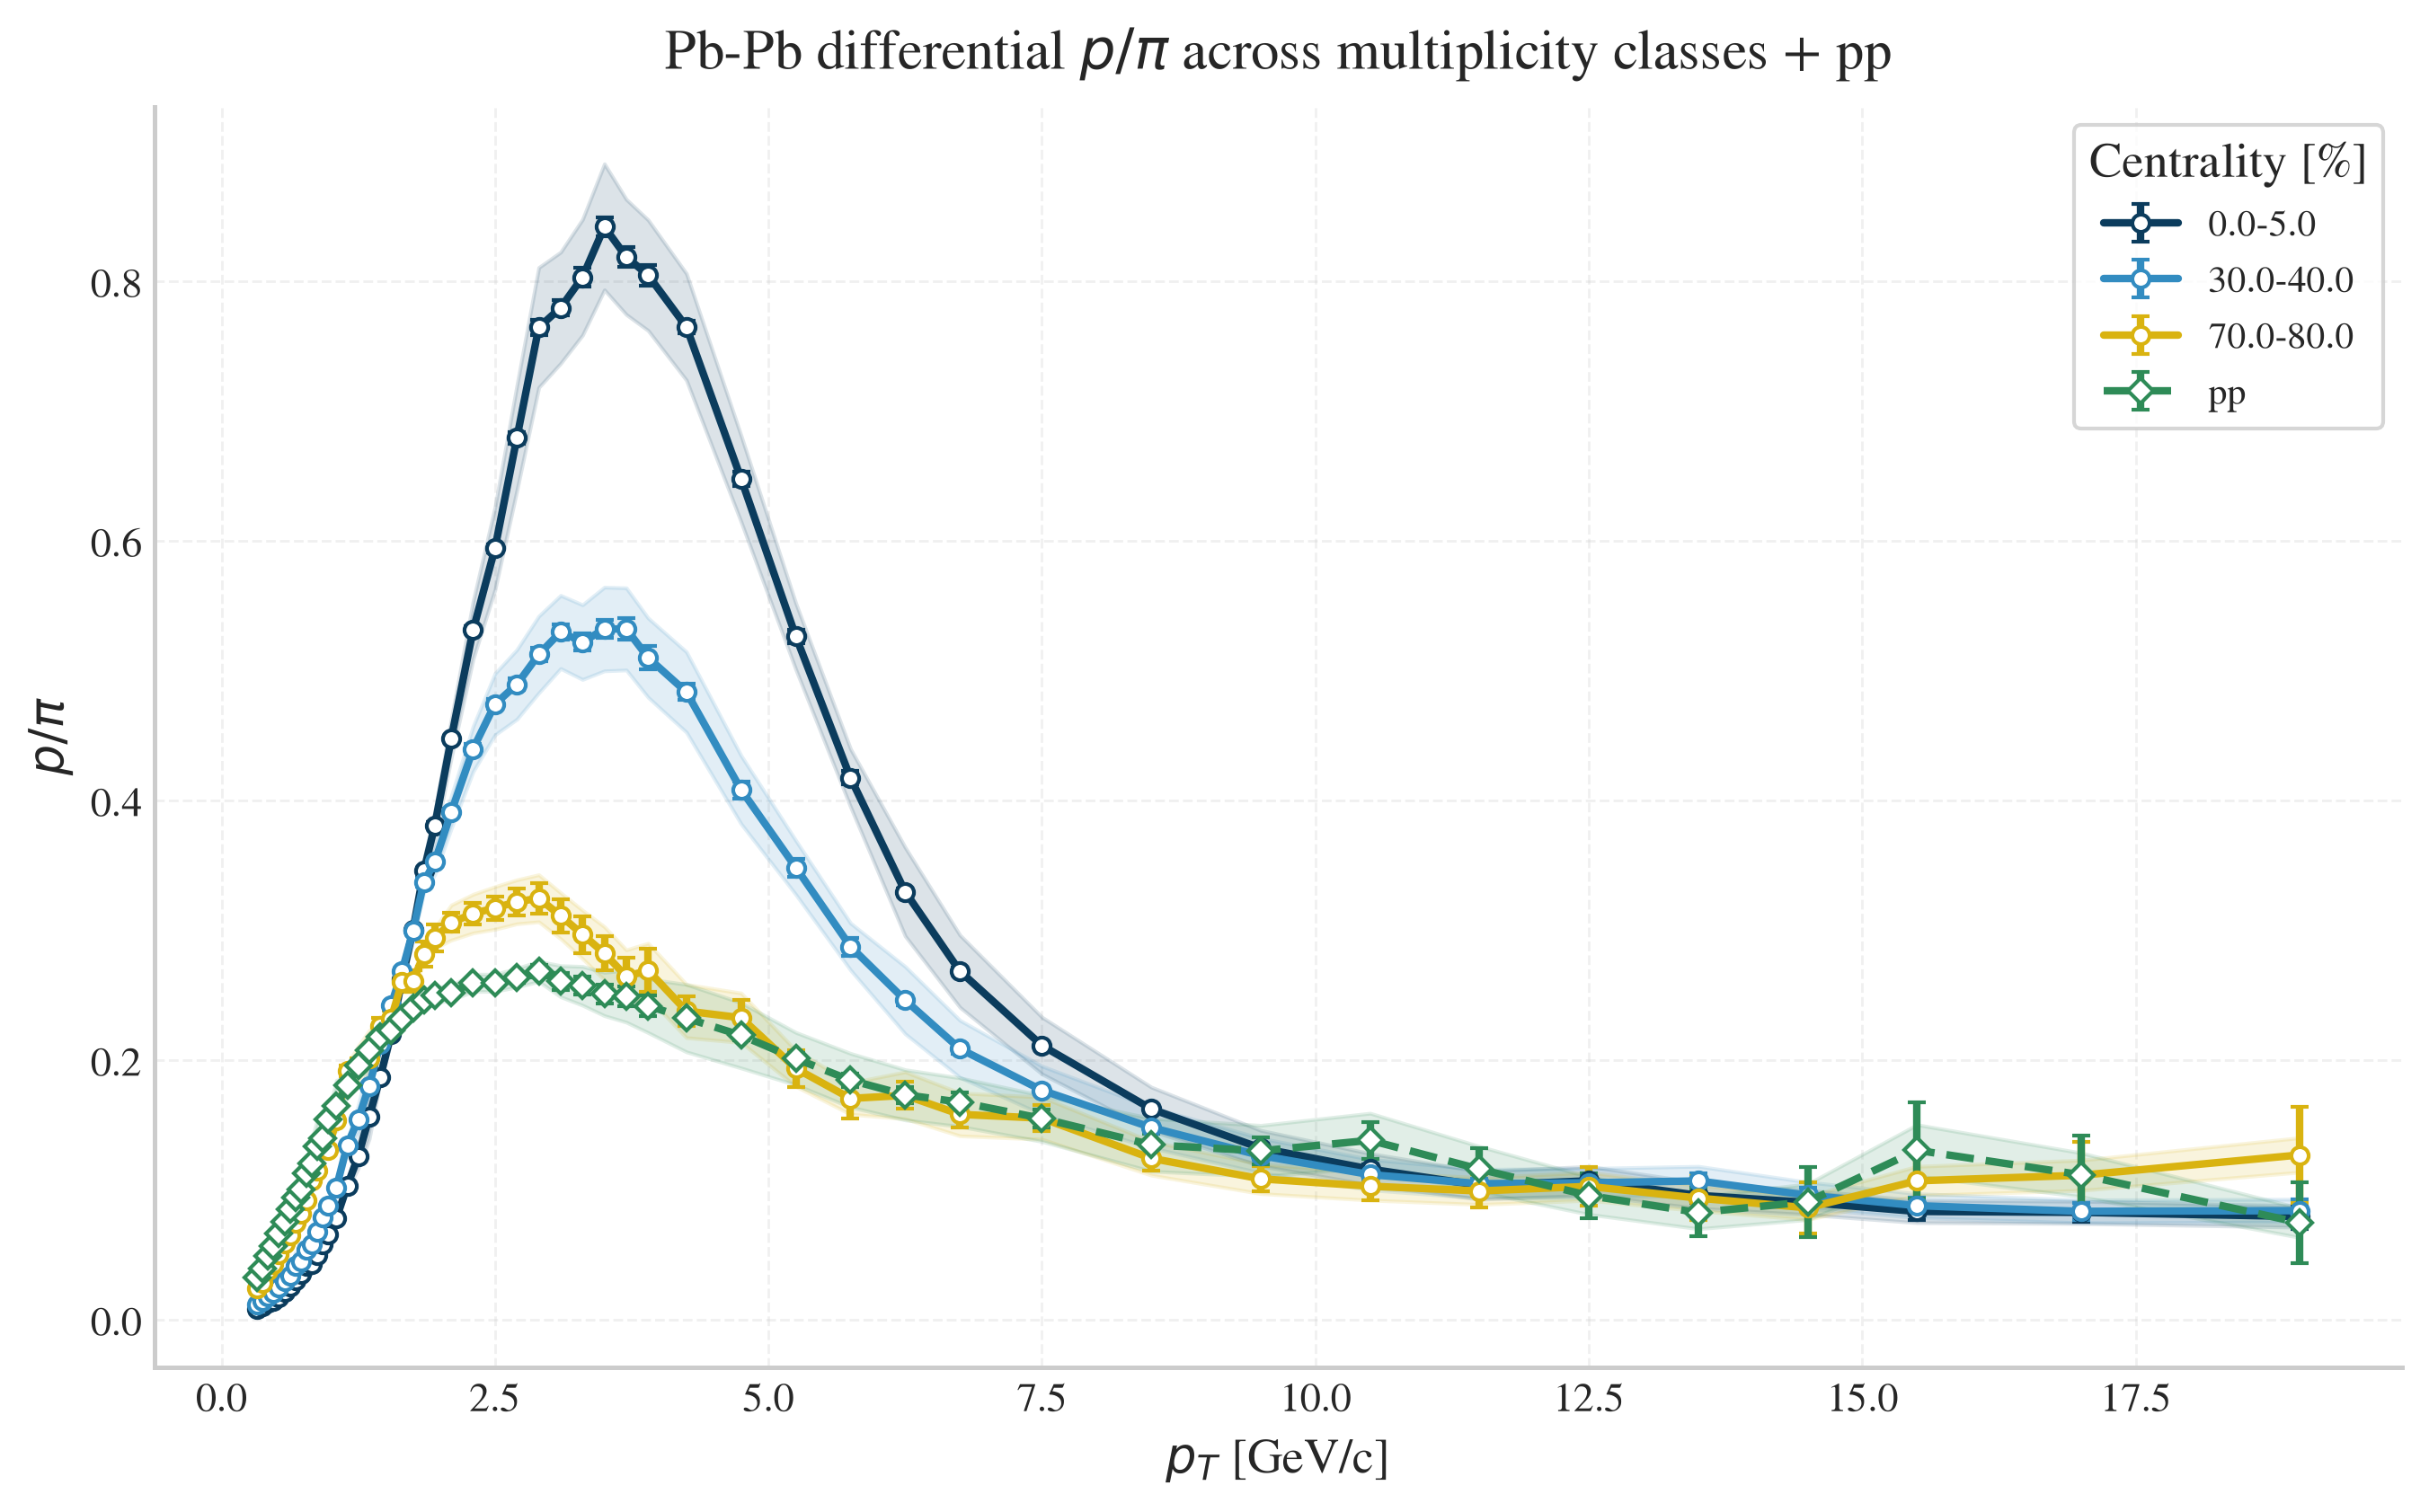
\includegraphics[
    width=\linewidth,
    height=0.45\textheight,
    keepaspectratio
]{img/qgp-enhancement.png}

\vspace{-0.3cm}
\begin{block}{Quark coalescence}
\small
The high quark density in the QGP favors hadronization by quark
recombination,
\[
qqq \rightarrow p,
\quad
q\bar q \rightarrow \pi ,
\]

enhancing baryon production relative to mesons at intermediate $p_T$.
\end{block}

\vspace{0.05cm}

{\tiny Differential $p/\pi$ ratio for different Pb--Pb centralities.}

\end{columns}

\vfill

\end{frame}